\chapter{Sprint 2 – Module Boutique}
	
\section*{Introduction}
Dans ce chapitre, nous allons nous intéresser à le module Boutique. Par la suite, nous nous intéresserons à l’aspect conceptuel et fonctionnel de ce sprint.

\section[Backlog sprint]{Backlog sprint}
Dans le backlog du sprint, nous présenterons deux parties :  le but du sprint et les user stories.

\subsection[But de sprint]{But de sprint}
En suivant le même principe que le sprint précédent, nous commencerons par définir l'objectif du sprint. Par conséquent, l'objectif de ce sprint est l'intégration de module Boutique et l’affectation des utilisateurs aux boutiques.
\subsection[User stories]{User stories}
Après avoir défini le but du sprint, nous pourrons lister les user stories qui appartiennent au sprint.
La table \ref{tab:user-stories-sprint-2} représente notre backlog de Sprint 2.
\begin{longtable}[c]{|l|l|l|}
	\hline
	\rowcolor[HTML]{C0C0C0} 
	User stories&
	Tâches &
	Complexité \\ \hline
	
	%
	\endhead
	%
	\begin{tabular}[c]{@{}l@{}}En tant qu’un administrateur, je\\ souhaite d’avoir toutes les \\ informations des boutiques à jour\end{tabular} &
	Intégrer le module Boutique dans le projet &
	1 \\ \hline
	\begin{tabular}[c]{@{}l@{}}En tant qu’un administrateur, je \\ souhaite d’affecter les utilisateurs\\ CPRO aux boutiques\end{tabular} &
	\begin{tabular}[c]{@{}l@{}}Ajouter les interfaces de la gestion\\ des affectations\\ \tabitem Consultation\\ \tabitem Modification\\ \tabitem Suppression\\ \tabitem Affectation des utilisateurs\\ \tabitem Recherche\\ et la logique derrière\end{tabular} &
	2 \\ \hline
	\begin{tabular}[c]{@{}l@{}}En tant qu’un administrateur, je\\ souhaite d’exporter les\\  affectations des utilisateurs CPRO\\  aux boutiques\end{tabular} &
	\begin{tabular}[c]{@{}l@{}}Ajouter bouton “exporter” dans\\ l’interface de gestion des\\ utilisateurs et la logique derrière\end{tabular} &
	3 \\ \hline
	\begin{tabular}[c]{@{}l@{}}En tant qu’un utilisateur de \\ Panoramix, je souhaite de simuler \\ la page SRCD\end{tabular} &
	Développer une interface SRCD &
	3 \\ \hline
	\captionsetup{justification=centering}
	\caption{User stories de sprint 2}
	\label{tab:user-stories-sprint-2}\\
\end{longtable}

\section{Etude de réalisation du sprint 2}
Cette section de notre projet présente les différents diagrammes de cas d’utilisation avec leurs raffinements
\subsection{Diagramme de cas d’utilisation global sprint 2}
La figure \ref{fig:usecase-sprint2} décrit le diagramme de cas d’utilisation global du sprint 2
\begin{figure}[H]
	\centering
	\includegraphics[width=0.7\linewidth]{"img/conception/usecases/sprint 2/UseCase-sprint2"}
	\caption[Diagramme de cas d’utilisation global sprint 2]{Diagramme de cas d’utilisation global sprint 2}
	\label{fig:usecase-sprint2}
\end{figure}
\subsection{Raffinement et description textuelle des diagrammes de cas d’utilisation}
Dans cette section, nous présentons les diagrammes des cas d’utilisation détaillés et leurs descriptions textuelles.
\newpage
\subsubsection{Description textuelle du cas d’utilisation «simulation SRCD»}
Le tableau suivant contient la description textuelle du cas d’utilisation «simulation SRCD»
\begin{table}[H]
	\centering
	\begin{tabular}{|l|l|}
		\hline
		\rowcolor[HTML]{C0C0C0} 
		Cas d’utilisation & simulation SRCD                        \\ \hline
		Acteurs           & Toute personne ayant l’accès à la page \\ \hline
		Résumé &
		\begin{tabular}[c]{@{}l@{}}Semble à la page bouchon qui sert à simuler le \\ mécanisme que le client est inscrit en entrant à \\ la boutique\end{tabular} \\ \hline
		Scénario principal &
		\begin{tabular}[c]{@{}l@{}}L’utilisateur remplit le formulaire par :\\ code edo de boutique\\ CUID de client \\ id d'établissement\end{tabular} \\ \hline
		Post condition    & Le client sera ajouté au fil d’attente \\ \hline
	\end{tabular}
	\captionsetup{justification=centering}
	\caption{ Description textuelle du cas d’utilisation «simulation SRCD»}
	\label{tab:descrip-text-sim-srcd}
\end{table}

\subsubsection{Description textuelle du cas d’utilisation «consultation boutiques»}
Le tableau \ref{tab:descrip-text-consult-boutique} contient la description textuelle du cas d’utilisation «consultation boutiques»
\begin{table}[H]
	\centering
	\begin{tabular}{|l|l|}
		\hline
		\rowcolor[HTML]{C0C0C0} 
		Cas d’utilisation & consultation boutiques                 \\ \hline
		Acteurs           & Administrateur                         \\ \hline
		Résumé &
		\begin{tabular}[c]{@{}l@{}}L’administrateur peut consulter les données \\ boutique via l’interface\end{tabular} \\ \hline
		Précondition      & L’administrateur doit être authentifié \\ \hline
		Scénario principal &
		\begin{tabular}[c]{@{}l@{}}L’administrateur accède à la page des données \\ boutique, il peut faire une recherche et il peut voir \\ toutes informations concernant une boutique\end{tabular} \\ \hline
	\end{tabular}
	\captionsetup{justification=centering}
	\caption{Description textuelle du cas d’utilisation «consultation boutiques»}
	\label{tab:descrip-text-consult-boutique}
\end{table}
\newpage
\subsubsection{Cas d’utilisation «affectation  utilisateurs aux boutiques»}
La figure \ref{fig:usecase-affectation} illustre le raffinement du cas d’utilisation «affectation utilisateurs aux boutiques»
\begin{figure}[H]
	\centering
	\includegraphics[width=0.7\linewidth]{"img/conception/usecases/sprint 2/UseCase-affectation"}
	\caption[Cas d’utilisation «affectation utilisateurs aux boutiques»]{Cas d’utilisation «affectation utilisateurs aux boutiques»}
	\label{fig:usecase-affectation}
\end{figure}
\myparagraph{Description textuelle du cas d’utilisation «affectation  utilisateurs aux boutiques»}
Le tableau \ref{tab:descrip-text-affect-user-boutique} contient la description textuelle du cas d’utilisation «affectation utilisateurs aux boutiques»
\begin{table}[H]
	\centering
	\begin{tabular}{|l|l|}
		\hline
		\rowcolor[HTML]{C0C0C0} 
		Cas d’utilisation & Affectation utilisateurs aux boutiques                        \\ \hline
		Acteurs           & Administrateur                                                \\ \hline
		Résumé            & L’administrateur peut affecter des utilisateurs aux boutiques \\ \hline
		précondition &
		\begin{tabular}[c]{@{}l@{}}l’administrateur doit être authentifié\\ L’utilisateur doit être existant\\ La boutique doit être existante\end{tabular} \\ \hline
		Scénario principal &
		\begin{tabular}[c]{@{}l@{}}Pour gérer les affectations, l’administrateur peut :\\ affecter un utilisateur à une boutique\\ Modifier une affectation\\ Supprimer une affectation\\ Consulter les affectations\\ Rechercher des affectations\end{tabular} \\ \hline
		Post condition    & Mettre à jour la liste des affectations                       \\ \hline
	\end{tabular}
	\captionsetup{justification=centering}
	\caption{Description textuelle du cas d’utilisation «affectation  utilisateurs aux boutiques»}
	\label{tab:descrip-text-affect-user-boutique}
\end{table}
\newpage
\subsubsection{Description textuelle du cas d’utilisation «mettre à jour les données boutiques»}
Le tableau \ref{tab:descrip-text-update-boutique} contient la description textuelle du cas d’utilisation «affectation utilisateurs aux boutiques»
\begin{table}[H]
	\centering
	\begin{tabular}{|l|l|}
		\hline
		\rowcolor[HTML]{C0C0C0} 
		Cas d’utilisation & Affectation utilisateurs aux boutiques \\ \hline
		Acteurs           & Système                                \\ \hline
		Résumé &
		\begin{tabular}[c]{@{}l@{}}Un script Bash sera exécuté chaque matin pour\\ exploiter les fichiers xml de serveur O3 afin d’obtenir\\ les nouvelles données boutiques\end{tabular} \\ \hline
		précondition &
		\begin{tabular}[c]{@{}l@{}}Chaque jour les fichiers O3 doit être existes dans le\\ dossier\end{tabular} \\ \hline
		Scénario principal &
		\begin{tabular}[c]{@{}l@{}}Le script sera lancé chaque matin et les fichiers O3\\ seront archivés avec leurs état ( soit OK en cas de\\ succès, soit KO en cas d'échec)\end{tabular} \\ \hline
		post condition    & Mettre à jour la liste des boutiques   \\ \hline
	\end{tabular}
	\caption{Description textuelle du cas d’utilisation «mettre à jour les données boutiques»}
	\label{tab:descrip-text-update-boutique}
\end{table}

\section{Conception}
Dans cette partie, nous présentons les différents diagrammes de classes ainsi que de séquence détaillés pour ce sprint.\newpage
\subsection{Diagramme de classes}
la figure \ref{fig:classdiag-sprint2} illustre la structure statique du sprint 2 schématisée dans un diagramme de classe globale.
\begin{figure}[H]
	\centering
	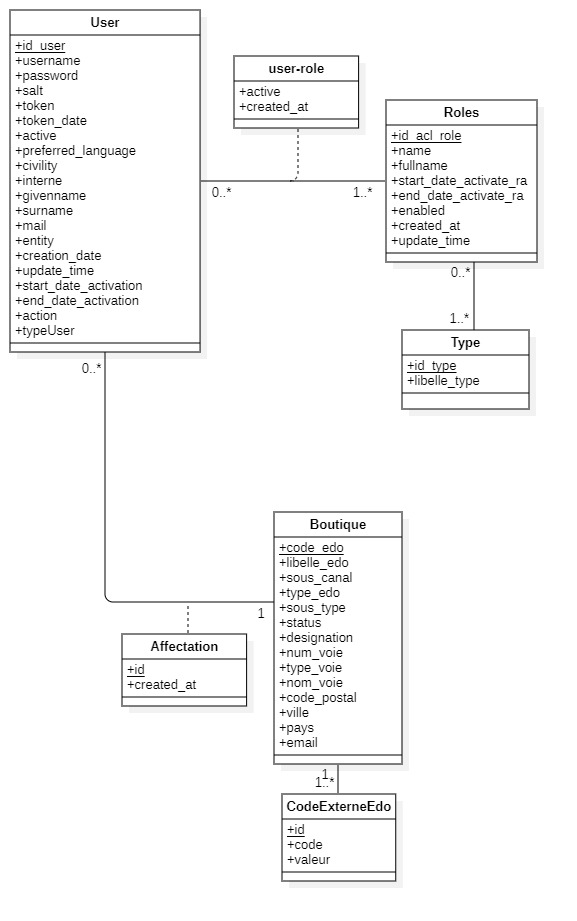
\includegraphics[width=0.5\linewidth]{img/conception/classes/ClassDiag-sprint2}
	\caption[Diagramme de classes de sprint 2]{Diagramme de classes de sprint 2}
	\label{fig:classdiag-sprint2}
\end{figure}

\subsection{Diagrammes de séquences détaillés}
Nous allons maintenant passer à l’aspect dynamique des opérations représentées dans le diagramme de classe à l’aide des diagrammes de séquences de système et d’objets.
\subsubsection[Quelques diagrammes de séquences système de Sprint 2]{Quelques diagrammes de séquences système de Sprint 2}
Dans cette section, nous présenterons quelques diagrammes de séquences système de “module Boutique” tels que :
\myparagraph{Diagramme de séquences système d’ «affecter un utilisateur au boutique»}
\begin{figure}[H]
	\centering
	\includegraphics[width=0.7\linewidth]{"img/conception/sequences/sprint 2/affectation-system"}
	\caption[Diagramme de séquences système d’ «affecter un utilisateur au boutique»]{Diagramme de séquences système d’ «affecter un utilisateur au boutique»}
	\label{fig:affectation-system}
\end{figure}

\myparagraph{diagramme de séquences objets d’ «affecter un utilisateur au boutique»}
\begin{figure}[H]
	\centering
	\includegraphics[width=0.65\linewidth]{"img/conception/sequences/sprint 2/affectation-obj"}
	\caption[diagramme de séquences objets d’ «affecter un utilisateur au boutique»]{diagramme de séquences objets d’ «affecter un utilisateur au boutique»}
	\label{fig:affectation-obj}
\end{figure}

\myparagraph{L'algorigramme de «mise à jour des données boutiques» }
\begin{figure}[H]
	\centering
	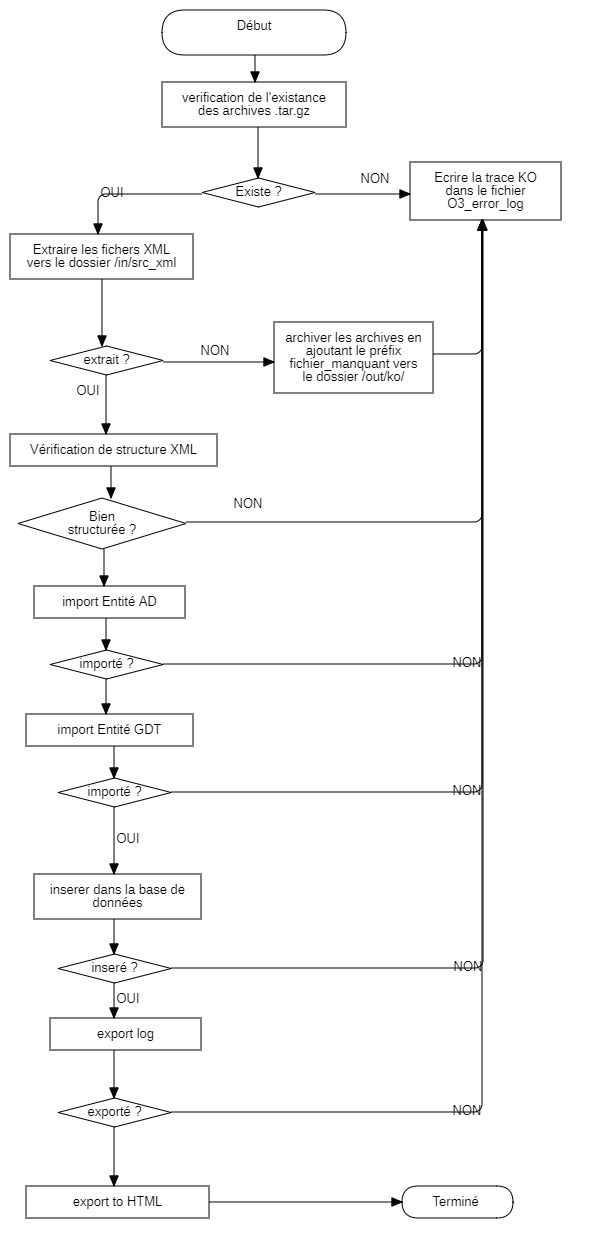
\includegraphics[width=0.6\linewidth]{img/conception/FlowchartDiagram-update-boutique}
	\caption[L'algorigramme de «mise à jour des données boutiques»]{L'algorigramme de «mise à jour des données boutiques»}
	\label{fig:flowchartdiagram-update-boutique}
\end{figure}

\section{Réalisation}
Dans cette sections nous allons exposer les différentes interfaces réalisées dans le sprint 2. 
\subsection{Interfaces de consultation boutique}
les captures d'écran ci-dessous représentent les deux IHMs de consultation boutique.
\begin{itemize}
	\item Consultation des boutiques et recherche
	\begin{figure}[H]
		\centering
		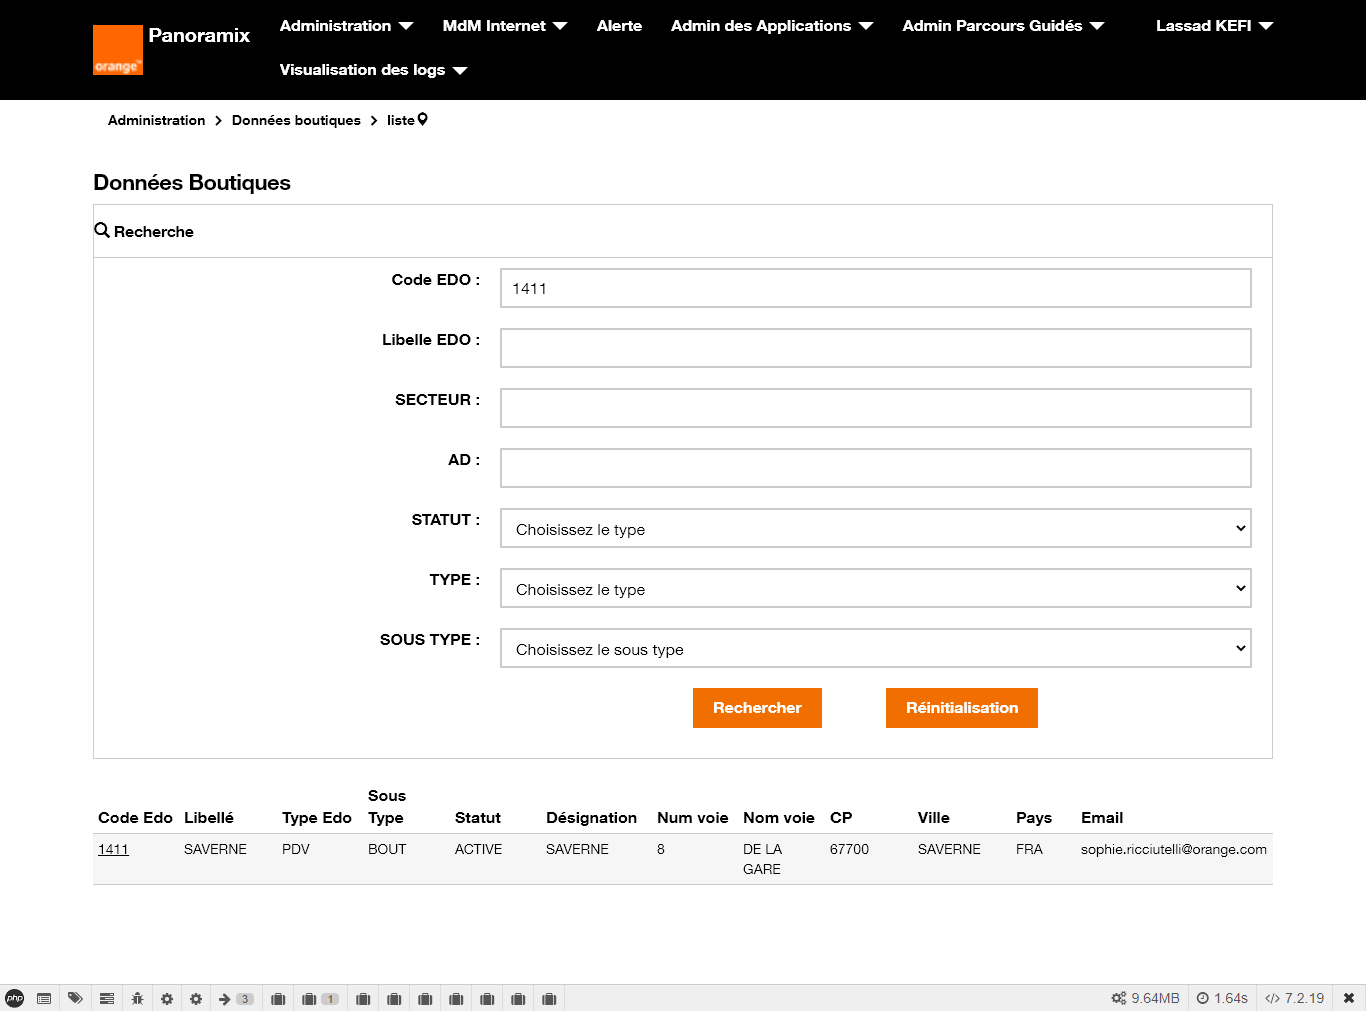
\includegraphics[width=0.5\linewidth]{img/screenshots/boutique/index}
		\caption[Interface consultation des boutiques et recherche]{Interface consultation des boutiques et recherche}
		\label{fig:index-btq}
	\end{figure}
	
	\item Voir les données d'une boutique
	\begin{figure}[H]
		\centering
		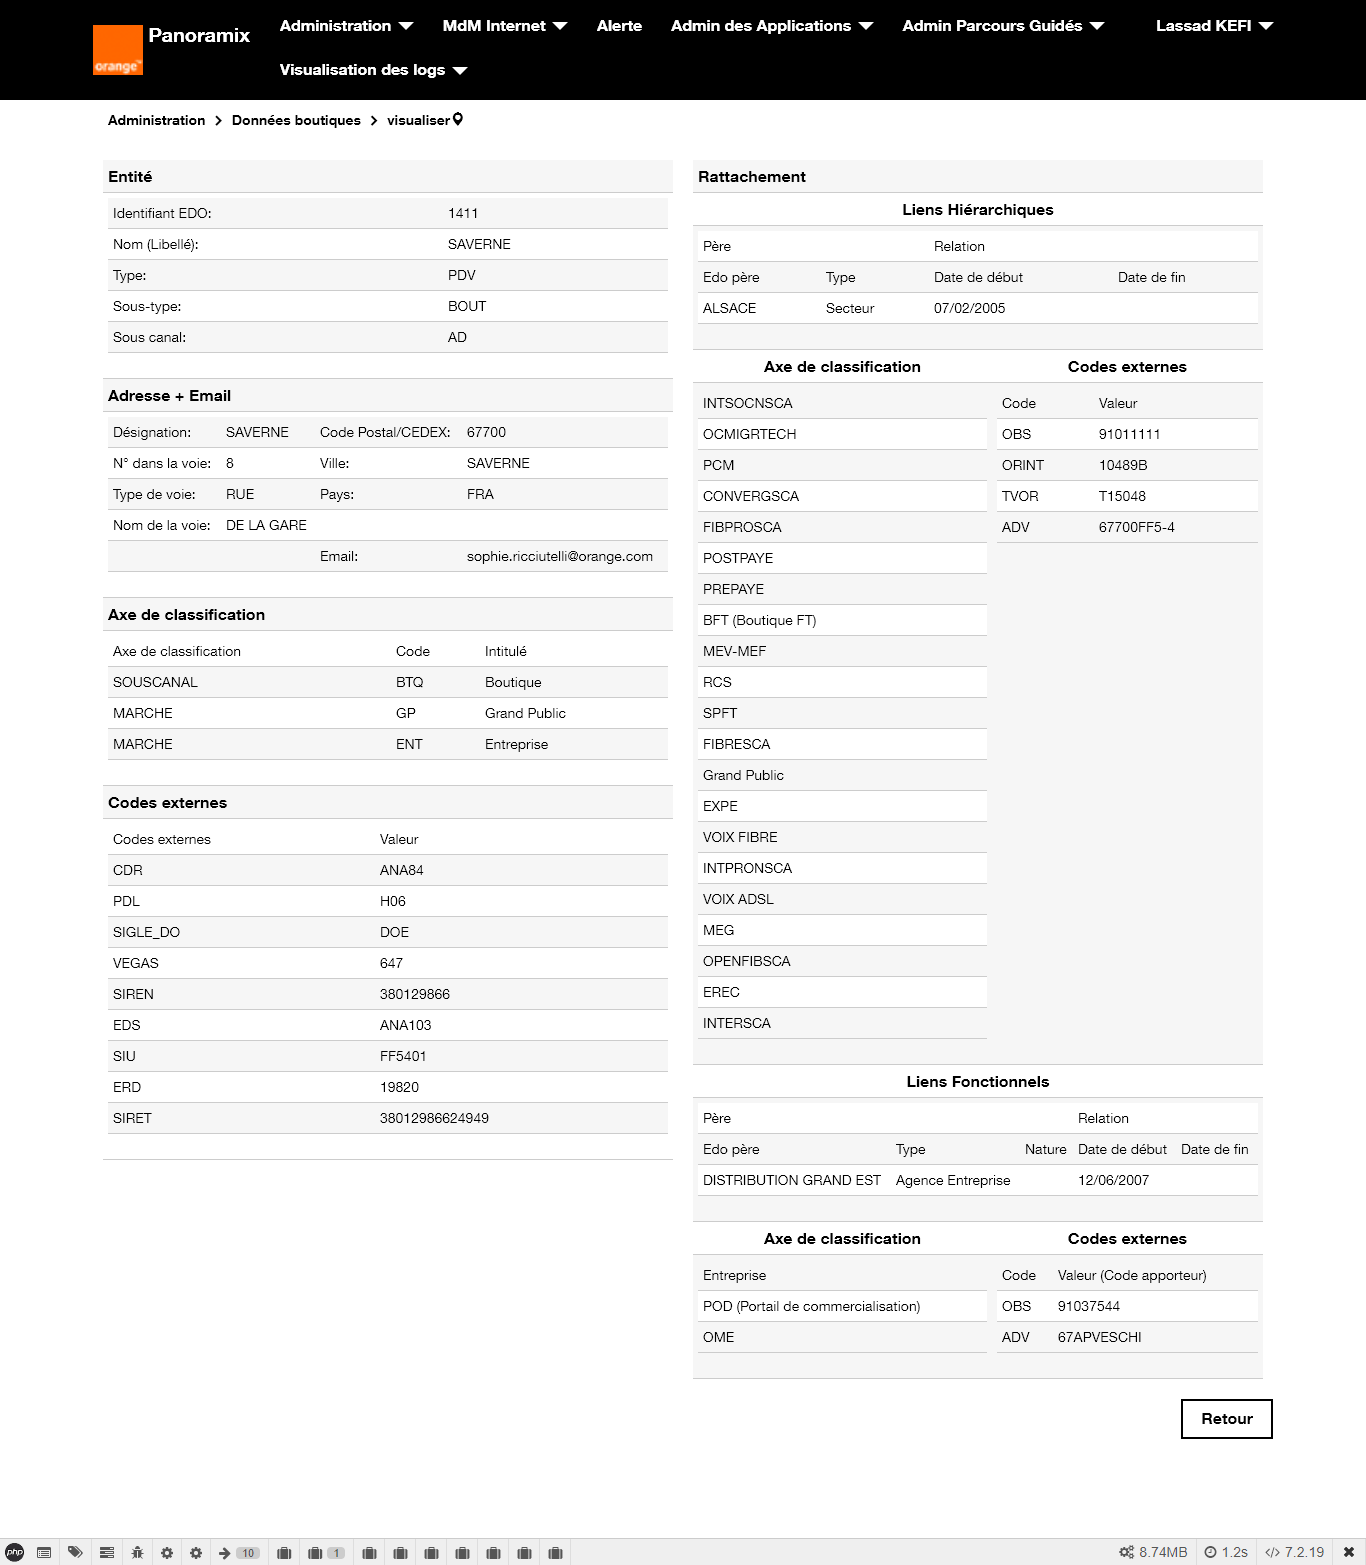
\includegraphics[width=0.5\linewidth]{img/screenshots/boutique/view}
		\caption[Interfacevoir les données d'une boutique]{Interface voir les données d'une boutique}
		\label{fig:view-btq}
	\end{figure}
\end{itemize}

\subsection{Interfaces de gestion des affectations}
les captures d'écran ci-dessous représentent les différentes IHM de gestion des affectations.
\begin{itemize}
	\item Consultation des affectations et recherche
	\begin{figure}[H]
		\centering
		\includegraphics[width=0.5\linewidth]{"img/screenshots/affectation users-boutique/index"}
		\caption[Interface consultation des affectations et recherche]{Interface consultation des affectations et recherche}
		\label{fig:index-affectation}
	\end{figure}
	
	\item Voir une affectation
	\begin{figure}[H]
		\centering
		\includegraphics[width=0.5\linewidth]{"img/screenshots/affectation users-boutique/view"}
		\caption[Interface voir une affectation]{Interface voir une affectation}
		\label{fig:view-affectation}
	\end{figure}

	\item Affecter un utilisateur à une boutique
	\begin{figure}[H]
		\centering
		\includegraphics[width=0.5\linewidth]{"img/screenshots/affectation users-boutique/affectation"}
		\caption[Interface affecter un utilisateur à une boutique]{Interface affecter un utilisateur à une boutique}
		\label{fig:create-affectation}
	\end{figure}

	\item Résultat d'exportation des affectations
	\begin{figure}[H]
		\centering
		\includegraphics[width=0.7\linewidth]{"img/screenshots/affectation users-boutique/export"}
		\caption[Interface résultat d'exportation des affectations]{Interface résultat d'exportation des affectations}
		\label{fig:export-affectation}
	\end{figure}
\end{itemize}
\subsection{Interface de simulation SRCD}
la capture d'écran ci-dessous représente l’interface de simulation SRCD.
\begin{figure}[H]
	\centering
	\includegraphics[width=0.7\linewidth]{"img/screenshots/logs + srcd/screencapture-localhost-pano-pfe-panoramix-public-srcd-phtml-2020-06-11-18_18_04"}
	\caption[Interface de simulation SRCD]{Interface de simulation SRCD}
	\label{fig:srcd}
\end{figure}

\section*{Conclusion}
Dans ce chapitre, nous avons terminé le troisième sprint, qui a permis l'intégration de “module Boutique” et la gestion des affectations en rédigeant sa conception. Dans le chapitre suivant, nous commençons le sprint final de notre projet.
